\begin{figure}[htbp]
  \centering
  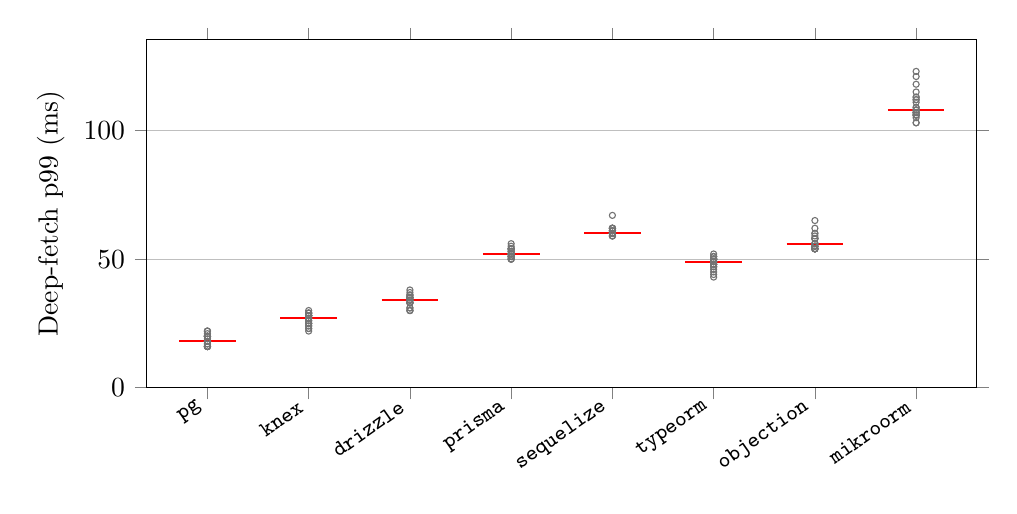
\begin{tikzpicture}
  \begin{axis}[width=\textwidth,height=6cm,
      ylabel={Deep-fetch p99 (ms)}, xmin=0.4, xmax=8.6, ymin=0,
      xtick={1,2,3,4,5,6,7,8}, xticklabels={\texttt{pg},\texttt{knex},\texttt{drizzle},\texttt{prisma},\texttt{sequelize},\texttt{typeorm},\texttt{objection},\texttt{mikroorm}},
      x tick label style={rotate=35,anchor=east,font=\footnotesize},
      ymajorgrids, tick align=outside]
  \addplot[only marks,mark=o,mark size=1.1pt,draw=black!55] coordinates {
(1,16) (1,18) (1,17) (1,22) (1,20) (1,18) (1,20) (1,16) (1,20) (1,19) (1,22) (1,22) (1,20) (1,18) (1,16) (1,18) (1,20) (1,17) (1,16) (1,16) (1,20) (1,20) (1,18) (1,16) (1,21)
(2,28) (2,24) (2,27) (2,27) (2,29) (2,23) (2,25) (2,29) (2,26) (2,26) (2,28) (2,29) (2,27) (2,30) (2,28) (2,25) (2,28) (2,25) (2,29) (2,28) (2,22) (2,24) (2,23) (2,28) (2,28)
(3,38) (3,33) (3,35) (3,30) (3,36) (3,33) (3,36) (3,30) (3,35) (3,34) (3,34) (3,35) (3,33) (3,30) (3,31) (3,36) (3,33) (3,31) (3,35) (3,33) (3,37) (3,34) (3,35) (3,34) (3,35)
(4,52) (4,54) (4,52) (4,53) (4,52) (4,54) (4,52) (4,51) (4,50) (4,51) (4,53) (4,52) (4,52) (4,51) (4,55) (4,54) (4,54) (4,51) (4,54) (4,50) (4,56) (4,50) (4,53) (4,50) (4,51)
(5,60) (5,60) (5,59) (5,60) (5,60) (5,59) (5,61) (5,60) (5,60) (5,62) (5,60) (5,62) (5,59) (5,61) (5,62) (5,60) (5,61) (5,62) (5,60) (5,60) (5,61) (5,62) (5,67) (5,60) (5,60)
(6,49) (6,50) (6,45) (6,50) (6,48) (6,48) (6,44) (6,49) (6,49) (6,43) (6,51) (6,47) (6,50) (6,50) (6,47) (6,51) (6,52) (6,50) (6,49) (6,50) (6,51) (6,50) (6,46) (6,48) (6,48)
(7,54) (7,58) (7,54) (7,56) (7,65) (7,56) (7,54) (7,55) (7,54) (7,58) (7,59) (7,60) (7,62) (7,58) (7,55) (7,58) (7,54) (7,56) (7,54) (7,54) (7,56) (7,60) (7,55) (7,55) (7,54)
(8,107) (8,106) (8,103) (8,108) (8,115) (8,123) (8,106) (8,109) (8,113) (8,109) (8,118) (8,112) (8,112) (8,113) (8,107) (8,107) (8,111) (8,106) (8,106) (8,103) (8,107) (8,105) (8,108) (8,121) (8,108)
  };
\addplot[thick,red,mark=none] coordinates {(0.72,18) (1.28,18)};
\addplot[thick,red,mark=none] coordinates {(1.72,27) (2.2800000000000002,27)};
\addplot[thick,red,mark=none] coordinates {(2.7199999999999998,34) (3.2800000000000002,34)};
\addplot[thick,red,mark=none] coordinates {(3.7199999999999998,52) (4.28,52)};
\addplot[thick,red,mark=none] coordinates {(4.72,60) (5.28,60)};
\addplot[thick,red,mark=none] coordinates {(5.72,49) (6.28,49)};
\addplot[thick,red,mark=none] coordinates {(6.72,56) (7.28,56)};
\addplot[thick,red,mark=none] coordinates {(7.72,108) (8.28,108)};
  \end{axis}
  \end{tikzpicture}
  \caption{The 25 per-run p99 values behind each reported deep-fetch p99 on PostgreSQL
    (red bar = median, the value tabulated in the main text). Each run's p99 is estimated from roughly
    the top 1\% of that run's requests, so a single run's p99 is noisy; the paper reports the
    \emph{median} of these 25 run-level p99 values with a within-campaign bootstrap interval rather than
    pooling dependent requests. The plot shows the run-to-run dispersion this median summarizes: it is
    tight for the fast layers and widens for the slower ones, consistent with the coarser p99 estimate
    at higher latency. A full per-request HDR recorder was not used (the load generator reports latency
    percentiles, not raw request latencies), so an HDR reconstruction is left to future work.}
  \label{fig:p99_spread}
\end{figure}
